%%%%%%%%%%%%%%%%%%%%%%%%%%%%%%%%%%%%%%%
\chapter*{Publications and author contributions}
\label{sec:pubs}
\addcontentsline{toc}{chapter}{PUBLICATIONS AND AUTHOR CONTRIBUTIONS}
%%%%%%%%%%%%%%%%%%%%%%%%%%%%%%%%%%%%%%%
In the course of satisfying the University of Arizona Department of Physics's requirements for a Ph.D. doctoral dissertation, I prepared the following publications which are reprinted in full in the appendices. These articles are not ordered chronologically, but in the contextual order of presentation in this document. My contribution to each work is described under each item.
\begin{itemize}
    \item \rapp{appendixA} - ``Magnetic dipole moment in relativistic quantum mechanics'' by~\citet*{Steinmetz:2018ryf} is a study and comparison of DP and KGP wave equations for homogeneous magnetic fields and hydrogen-like atoms. I performed all computation, writing, and figure making in preparation of the first draft and approved the final draft before submission. I acknowledge the help and consultation of Martin Formanek (MF) and Johann Rafelski (JR) in research, writing and editing.
    \item \rapp{appendixB} - ``Strong fields and neutral particle magnetic moment dynamics'' by~\citet*{Formanek:2017mbv} is an overview of our research group's efforts in studying neutral particle dynamics in electromagnetic fields. I wrote Section 2.1 in collaboration with MF. I consulted and helped lead author MF and co-authors Stefan Evans (SE) and Cheng Tao Yang (CTY) in editing and revising the overall manuscript.
    \item \rapp{appendixC} - ``Relativistic dynamics of point magnetic moment'' by~\citet*{Rafelski:2017hce} introduces a new covariant formulation of classical spin dynamics and unifies Gilbertian and Amp{\`e}rian dipoles. I wrote Section 3 in collaboration with JR and MF and aided in the computation in Section 5.1. I otherwise consulted in the research, writing, and editing process of this publication.
    \item \rapp{appendixD} - ``Dynamic fermion flavor mixing through transition dipole moments'' by \citet*{Rafelski:2023aaa} is a study of Majorana neutrino flavor mixing in electromagnetic fields and proposes a novel effective EM-mass basis for propagating neutrinos. The article was written originally via invitation of JR by Gerhard Buchalla, Dieter L\"ust and Zhi-Zhong Xing as a memorial chapter in a book dedicated to Harald Fritzsch. I performed all computation and writing in preparation of the first draft and approved the final draft before submission. I acknowledge the help and consultation of JR and CTY in research, writing and editing.
    \item \rapp{appendixE} - ``A Short Survey of Matter-Antimatter Evolution in the Primordial Universe'' by~\citet*{Rafelski:2023emw} is a 50 page long review with many novel results describing the role of antimatter in the early universe. I supervised (in collaboration with CTY) the document creation, combining the writing contributions of all authors (including myself, Jeremiah Birrell (JB), CTY, and JR) into one coherent presentation. I also coordinated with all authors in formatting and editing the technical figures in this review by JB, CTY, and JR.
    \item \rapp{appendixF} - ``Matter-antimatter origin of cosmic magnetism'' by~\citet*{Steinmetz:2023nsc} proposes a model of para-magnetization driven by the large matter-antimatter (electron-positron) content of the early universe. I carried out all writing in preparation of the first draft and approved the final draft before submission. Computation and figure making was done in collaboration with CTY who contributed key results and five technical figures. I acknowledge the help and consultation of CTY and JR in research, writing and editing.
\end{itemize}

This is not a total catalogue of my research efforts, but lists the works that form the foundation of \rchap{chap:moment}, \rchap{chap:neutrino} and \rchap{chap:cosmo} of this dissertation. Where noted, these chapters also contain sections of complete yet unpublished work. \rchap{chap:outlook} contains brief discussions of still-in-progress research efforts to be completed after submission of this dissertation.

I was also co-author on the following publications which are not used extensively in this dissertation and are not reprinted as appendices. They are listed in chronological order below. In these three works I consulted with MF and JR in research and editing making content clarifying contributions to these manuscripts:
\begin{itemize}
    \item ``Classical neutral point particle in linearly polarized EM plane wave field'' by~\citet*{Formanek:2019cga} explores the dynamical equations presented in \rapp{appendixC} for neutral particles with magnetic moment.
    \item ``Radiation reaction friction: Resistive material medium'' by~\citet*{Formanek:2020zwc} introduces a novel model of relativistic covariant friction within a medium.
    \item ``Motion of classical charged particles with magnetic moment in external plane-wave electromagnetic fields'' by~\citet*{Formanek:2021mcp} is a followup to the above 2019 work and \rapp{appendixC} for charged particles with magnetic moment.
\end{itemize}

%%%%%%%%%%%%%%%%%%%%%%%%%%%%%%%%%%%%%%%
\chapter{The importance of spin}
\label{chap:intro}
%%%%%%%%%%%%%%%%%%%%%%%%%%%%%%%%%%%%%%%
\noindent All fundamental particles known in physics have a non-zero quantized spin angular momentum with the exception of the Higgs boson which is a scalar with spin-0. All other confirmed elementary particles (such as electrons, quarks, photons, etc...) have values of either spin-1/2 or spin-1. Particles with even values of spin are known as bosons while half-integer particles with spin are called fermions. Composite particles (such as atomic nuclei) can exhibit more exotic spin values and fundamental particles with higher spins such as spin-3/2 or spin-2 graviton are commonly predicted in beyond-standard-model (BSM) physics.

In the realm of the Poincar{\'e} group of spacetime symmetry (rotations, boosts and translations) transformations, each particle can be uniquely labeled by two distinct Casimir invariants: mass and spin. These two operators commute with all generators of the Poincar{\'e} group and act as labels which represent a particle. Therefore in a relativistic context, particle mass and spin are of fundamental importance on equal footing.

If a particle is electrically charged, then by virtue of its spin it will have a magnetic dipole moment. Most neutral particles with spin, though not all, will also have magnetic dipoles though for more complex reasons. Therefore the magnetic behavior of particle is an important window into probing one of the most fundamental properties in physics. As quantum mechanics is not well described in terms of forces or accelerations (except in the context of Ehrenfest-style equations), there is no simple operator description of torque and spin-forces despite having played a key role in the development of quantum mechanics. For a short historical overview of spin see~\cite{Ohanian:1986wg}.

This introduction serves to motivate the fundamental concepts of spin, magnetic moment and electromagnetism which have played a crucial role in the history physics and will be explored in the subsequent research chapters. Magnetic (and electric) dipoles, anomalous magnetic moments (AMM), and the wave equations which describe spin-1/2 fermions are covered in \rsec{sec:mom}. Lastly, \rsec{sec:flrw} covers topics in $\Lambda\mathrm{CDM}$ cosmology which are particular relevance to \rchap{chap:cosmo}. This chapter will also serve to establish notation and mathematical conventions. SI units will be used unless otherwise stated.

%The classical connection between quantum operators, force and torque will be discussed in \rsec{sec:ehrenfest}.

%; see \rsec{sec:ehrenfest}

%%%%%%%%%%%%%%%%%%%%%%%%%%%%%%%%%%%%%%%
\section{Quantum magnetic dipoles and wave equations}
\label{sec:mom}
%%%%%%%%%%%%%%%%%%%%%%%%%%%%%%%%%%%%%%%
In classical theory, when charges rotate or circulate in some manner, a magnetic field is produced characterized by the magnetic dipole moment of the system. An Amp{\`e}rian loop of wire with a current is the quintessential example. This concept can be transplanted into quantum theory for spinning particles where the natural size of the magnetic moment of a particle (in this context a charged lepton) is given by the magneton value
\begin{gather}
    \label{mag:1}
    \mu_{\ell}\equiv\frac{e\hbar}{2m_{\ell}}
\end{gather}
where the lepton (denoted by $\ell$) has charge $e$ and mass $m_{\ell}$. 

A quick word on notation: Euclidean three-vectors and matrices will be denoted by boldface font. If indices are specifically printed, they will be done so using Latin indices such as $s_{i}$. Inner products of three-vectors will be noted via $\bb{a}\cdot\bb{b}=a_{i}b_{i}$ using Einstein summation notation where repeated indices are summed over. For electrons, \req{mag:1} is referred to as the Bohr magneton $\mu_{B}$. The non-relativistic spin operator $\bb{S}$ for a spin-1/2 particle is defined as
\begin{gather}
    \label{qspin:1}
    \bb{S}=\frac{\hbar}{2}\bb{\sigma}=\frac{\hbar}{2}\left(\sigma_{1},\,\sigma_{2},\,\sigma_{3}\right)^\mathrm{T}\,,
\end{gather}
where $\bb{\sigma}$ is the three-vector comprised of the familiar $2\times2$ Pauli matrices which act upon two-component spinors $\chi=(\chi_{1},\chi_{2})^\mathrm{T}$. Spinor indices will be suppressed or noted with Latin indices. The algebra defined by the commutators of the Pauli matrices serves as a representation of $SU(2)$ group structure
\begin{gather}
    \label{pauli:1}
    \{\sigma_{i},\sigma_{j}\}=2\delta_{ij}\,,\qquad
    [\sigma_{i},\sigma_{j}] = 2i\varepsilon_{ijk}\sigma_{k}\,,
\end{gather}
where $\varepsilon_{ijk}$ is the totally antisymmetric Levi-Civita symbol and $\delta_{ij}$ is the Kronecker delta.

The relativistic theory of spin-1/2 fermions however necessitates a four-component spinor $\psi=(\psi_{1},\psi_{2},\psi_{3},\psi_{4})^\mathrm{T}$ which as Dirac famously noted accommodates the required degrees of freedom for particles and antiparticles as well as both spin up $(\uparrow)$ and spin down $(\downarrow)$ eigenstates. The Hamiltonian density (in the Dirac representation) for the magnetic dipole moment interaction is given by
\begin{gather}
	\label{pauli:2}
    \mathcal{H}_\mathrm{int} = \frac{e\hbar}{2m_{\ell}}\psi^{\dag}
    \begin{pmatrix}
        -\bb{\sigma}\cdot\bb{B} & i\bb{\sigma}\cdot\bb{E}/c\\
        -i\bb{\sigma}\cdot\bb{E}/c & \bb{\sigma}\cdot\bb{B}
    \end{pmatrix}
    \psi\,,
\end{gather}
where $\psi^{\dag}$ is the complex conjugate transpose of the $\psi$ spinor. The electric $\bb{E}$ and magnetic $\bb{B}$ fields are defined in terms of the scalar potential $V$ and vector potential $\bb{A}$ in the usual way.
\begin{align}
    \label{eb:1}
    \bb{E}=-\bb{\nabla}V-\frac{\partial\bb{A}}{\partial t}\,,\qquad
    \bb{B}=\bb{\nabla}\times\bb{A}\,.
\end{align}

In the non-relativistic limit for particle states, the lower (antiparticle) components of $\psi$ suppressed by $|\bb{p}|/mc$ which we can approximate to first order as
\begin{align}
    \label{approx:1}
    \psi\approx\left(\chi,\ \frac{\bb{\sigma}\cdot\bb{\pi}}{2m_{\ell}c}\chi\right)^\mathrm{T}\,,\qquad \bb{\pi}=\bb{p}-e\bb{A}\,.
\end{align}
The operator $\bb{\pi}$ is the kinetic momentum operator written in terms of canonical momentum $\bb{p}$ and vector potential $\bb{A}$. Making use of the identity
\begin{align}
    \sigma_{i}\sigma_{j} = \delta_{ij} + i\varepsilon_{ijk}\sigma_{k}\,,
\end{align}
we insert \req{approx:1} into \req{pauli:2} yielding to order $\mathcal{O}(1/m^{3})$
\begin{gather}
    \label{ham:1}
    \mathcal{H}_\mathrm{int} \approx -\chi^{\dag}\left(\frac{e\hbar}{2m_{\ell}}\bb{\sigma}\cdot\bb{B}
    +\frac{ie\hbar}{4m_{\ell}^{2}c^{2}}\Big[(\bb{\sigma}\cdot\bb{E}),(\bb{\sigma}\cdot\bb{\pi})\Big]\right)\chi\\
    \label{ham:2}
    \mathcal{H}_\mathrm{int} \approx -\chi^{\dag}\left(\frac{e\hbar}{2m_{\ell}}\bb{\sigma}\cdot\bb{B}
    +\frac{e\hbar^{2}}{4m_{\ell}^{2}c^{2}}\bb{\nabla}\cdot\bb{E}
    +\frac{e\hbar}{4m_{\ell}^{2}c^{2}}\bb{\sigma}\cdot\left(\bb{E}\times\bb{\pi}-\bb{\pi}\times\bb{E}\right)\right)\chi\,.
\end{gather}
Keeping only up to first order, the dipole interaction \req{pauli:2} reduces to 
\begin{gather}
	\label{pauli:3}
    \mathcal{H}_\mathrm{int} \approx -\frac{e\hbar}{2m_{\ell}}\chi^{\dag}\bb{\sigma}\cdot\bb{B}\chi\,,
\end{gather}
which is the expected non-relativistic quantum dipole term. The second and third terms in \req{ham:2} can be interpreted as a Darwin term $\sim\bb{\nabla}\cdot\bb{E}$ sensitive to charge density and spin orbit coupling $\sim\bb{\sigma}\cdot(\bb{E}\times\bb{p})$. We will return to relativistic notation and concepts in \rsec{sec:dp}.

The magnetic moment operator $\bb{\mu}$, as suggested by \req{pauli:3} is defined in terms of the Pauli matrices as
\begin{gather}
    \label{mag:3}
    \bb{\mu}=g\left(\frac{e\hbar}{2m_{\ell}}\right)\frac{\bb{\sigma}}{2}=g\mu_{\ell}\frac{\bb{\sigma}}{2}\,,\qquad\mu\equiv\frac{g}{2}\mu_{\ell}\,,
\end{gather}
where $\mu$ is the `total magneton' value representing the full magnetic moment. The parameter $g$ in \req{mag:3} is the gyromagnetic ratio (or $g$-factor) of the particle. The `natural' value is $g\!=\!2$. While this prediction is normally attributed to the Dirac equation, it justified from the construction of the kinetic energy operator in the Schr{\"o}dinger-Pauli equation; see \rsec{sec:unique} and~\cite{sakurai1967advanced}.

In non-relativistic quantum mechanics, the time-dependant Schr{\"o}dinger-Pauli (SP) equation (with Hamiltonian $H_\mathrm{SP}$) for a charged particle is given by
\begin{gather}
	\label{sp:1}
    {H}_{\mathrm{SP}}\chi=\left(\frac{1}{2m_{\ell}}\bb{\pi}^{2}-\bb{\mu}\cdot\bb{B}+e{ V}\right)\chi=i\hbar\frac{\partial}{\partial t}\chi\,,\qquad
    \bb{\pi}=\bb{ p}-e{\bb{A}}\,,
\end{gather}
where $\chi$ is again a two-component spinor. It is well known that \req{sp:1} is obtainable from the Dirac equation (see \rsec{sec:dp}) in the non-relativistic limit.

Before moving on, we will verify that the SP \req{sp:1} contains within it an expression of the Stern-Gerlach force which was used to first provide evidence of the quantization of angular momentum~\citep{Gerlach:1922zz}. To accomplish this, we will work in the Heisenberg representation where operators obey the following equation of motion
\begin{align}
    \label{h:1}
    i\hbar\frac{d\bb{O}}{dt}=[\bb{O},H]+
    i\hbar\frac{\partial\bb{O}}{\partial t}\,,
\end{align}
To obtain a `force' in quantum mechanics we need to find the time derivative of the kinematic momentum operator $\bb{\pi}$ which is given by
\begin{gather}
    \label{h:2}
    \frac{d\bb{\pi}}{dt}=-\frac{i}{\hbar}[\bb{\pi},H_\mathrm{SP}]+\frac{\partial\bb{\pi}}{\partial t}=-\frac{i}{\hbar}\left[\bb{\pi},\frac{(\bb{\sigma}\cdot\bb{\pi})^{2}}{2m}+eV\right]+\frac{\partial\bb{\pi}}{\partial t}\,,\\
    \label{h:3}
    \frac{\partial\bb{\pi}}{\partial t} = -\frac{\partial e\bb{A}}{\partial t}\,,\qquad
    [\pi_{i},\pi_{j}]=ie\hbar\varepsilon_{ijk}B_{k}\,,\qquad
    [\pi_{i},B_{j}]=-i\hbar\nabla_{i}B_{j}\,.
\end{gather}
After some derivation and making use of the identities in \req{h:3}, we arrive at the quantum analog of the Lorentz force for particles with spin
\begin{gather}
    \label{ehren:1}
    \boxed{\frac{d\bb{\pi}}{dt}=e\bb{E}+\frac{e}{2m}(\bb{\pi}\times\bb{B}-\bb{B}\times\bb{\pi})+\frac{e\hbar}{2m}\sigma_{i}\bb{\nabla}B_{i}}\,.
\end{gather}
The last term in the expression is the Stern-Gerlach force which is sensitive to inhomogeneous magnetic fields. We also note this equation is suggestive of the `Amp{\'e}rian' dipole force which is in the direction of the gradient $\bb{\nabla}$ rather than the `Gilbertian' type of dipole force which is in the direction of the field $\bb{B}$; see \rsec{sec:cspin}. \req{ehren:1} can be connected to our classical understanding by taking the expectation value and casting it as an Ehrenfest-style theorem~\citep{Ehrenfest:1927swx}.

\subsection{Anomalous magnetic moment}
In nature there is no particle with exactly $g\!=\!2$. As seen in \rt{tab:gfactor}, composite particles often deviate from $g\!=\!2$ greatly as the $g$-factor of a composite particle is related to its internal composition. In the case of the neutron and proton, the internal quarks themselves are responsible. The comparison between three listed isotopes of hydrogen also displays how magnetic moments can `cancel out' or add together. While deuterium's value of $g$ is suppressed by the extra neutron, the two neutrons in tritium balance one another returning the ratio into one manifestly similar to the proton.

When $g\neq2$ (which is true for all physical particles with magnetic moment; composite of otherwise) the anomalous magnetic moment (AMM) can be defined via 
\begin{gather}
    \label{amm:1}
    a\equiv\frac{g}{2}-1\,,\qquad
    a\frac{e\hbar}{2m_{\ell}}\rightarrow\delta\mu\equiv\mu-\mu_{\ell}\,,
\end{gather}
where $a$ is the anomaly parameter. We also introduce $\delta\mu$ as the anomalous magneton which will be helpful in our proposal to connect mass and magnetic moment in \rsec{sec:ikgp} and \rsec{sec:numoment}.

\begin{table}
	\centering
\begin{tabular}{r|c|l}
    particle & category & $g$-factor\\
    \hline
	electron & elementary & -2.002\ 319\ 304\ 362\ 56(35)\\
	muon & elementary & -2.002\ 331\ 8418(13)\\
	tau & elementary & -2.036(34)\\
	neutron & composite & -3.826\ 085\ 45(90)\\
	proton & composite & \ 5.585\ 694\ 6893(16)\\
	deuterium & composite & \ 0.857\ 438\ 2338(22)\\
	tritium & composite & \ 5.957\ 924\ 931(12)\\
\end{tabular}
	\caption{The $g$-factor of various particles found in~\cite{ParticleDataGroup:2022pth}.}
	\label{tab:gfactor}
\end{table}

The anomalous magnetic moment of a particle can arise from a variety of physical sources with the most famous being the one-loop vacuum polarization contribution to the electron first computed by~\cite{Schwinger:1951nm}. In that work, the first correction to $g$ is given by
\begin{gather}
    a_{e} = \frac{\alpha}{2\pi}\,,\qquad
    \alpha\equiv\frac{1}{4\pi\varepsilon_{0}}\frac{e^{2}}{\hbar c}\,,
\end{gather}
where $\alpha$ is the fine structure constant with an approximate value of $1/137$. The measurement of the electron's $g$-factor is among the most precise measurements in all of physics~\citep{Tiesinga:2021myr} and rapid advancements in the measurement of the muon's anomalous magnetic moment have been announced even just prior to this dissertation being finalized~\citep{Muong-2:2023cdq}. This makes the study of magnetic moment, and spin, an exciting area of physical research as new developments continue today.

%%%%%%%%%%%%%%%%%%%%%%%%%%%%%%%%%%%%%%%
\subsection{Dirac and Dirac-Pauli equations}
\label{sec:dp}
%%%%%%%%%%%%%%%%%%%%%%%%%%%%%%%%%%%%%%%
\noindent While it is always beneficial to be well-appraised of non-relativistic mechanics, nature is intrinsically relativistic and therefore this dissertation must be as well. The relativistic generalization of \req{sp:1} is the Dirac equation given by
\begin{gather}
    \label{dirac:1a}
    \left(\gamma_{\alpha}\left(i\hbar\partial^{\alpha} - eA^{\alpha}\right)-m_{\ell}c\right)\psi=0\,,\\
    \label{dirac:1b}
    \pi^{\alpha}=i\hbar{\widetilde\nabla}^{\alpha}=i\hbar\partial^{\alpha}-eA^{\alpha}\,.
\end{gather}
The wave function $\psi$ in \req{dirac:1a} is understood to be a four-component spinor and $\widetilde\nabla^{\alpha}$ in \req{dirac:1b} is the covariant derivative. $\pi^{\alpha}$ is the four-vector version of the kinetic momentum versus the four-momentum $p^{\alpha}=i\hbar\partial^{\alpha}$. Four-vectors and tensors in this work will be denoted by Greek indices. Inner products of four-vectors will be noted by $a\cdot b=a^{\alpha}\eta_{\alpha\beta}b^{\beta}=a^{\alpha}b_{\alpha}$ again following Einstein notation. The four-derivative $\partial^{\alpha}$ and four-potential $A^{\alpha}$ are defined as
\begin{gather}
    \label{dirac:2}
    \partial^{\alpha}=\left(\frac{1}{c}\frac{\partial}{\partial t},\,-\bb{\nabla}\right)\,,\qquad A^{\alpha}=\left(\frac{V}{c},\,\bb{A}\right)\,.
\end{gather}
We have written the Dirac equation here in the covariant form where $\gamma^{\alpha}$ are the gamma matrices which obey the anticommuting Clifford algebra
\begin{gather}
    \label{gamma:1}
    \{\gamma_{\alpha},\gamma_{\beta}\}=\gamma_{\alpha}\gamma_{\beta} + \gamma_{\beta}\gamma_{\alpha} = 2\eta_{\alpha\beta}\,,\\
    \eta_{\alpha\beta}=\mathrm{diag}(+1,-1,-1,-1)\,,
\end{gather}
where $\eta_{\alpha\beta}$ is the flat spacetime Minkowski metric tensor defined with a positive time metric signature. The metric tensor is also responsible for raising and lowering covariant and contravariant indices e.g. $a_{\alpha}=\eta_{\alpha\beta}a^{\beta}$. As $\gamma^{\alpha}$ are also spinor matrices, the commutator in \req{gamma:1} carries implicit spinor indices which here computes to the $4\times4$ identity matrix $\mathbbm{1}_{4}$ (which is suppressed). We also introduce the `fifth' gamma matrix $\gamma^{5}$ which anticommutes with $\gamma^{\alpha}$ and the following standard conventions following~\cite{Itzykson:1980rh}
\begin{alignat}{1}
	\label{conventions:1} \bb{\alpha}=\gamma^{0}\bb{\gamma}\,,\indent \bb{\Sigma}=\gamma^{5}\bb{\alpha}\,,\indent \gamma^{5}=i\gamma^{0}\gamma^{1}\gamma^{2}\gamma^{3}\,,\indent \gamma^{2}_{5}=1\,.
\end{alignat}

As mentioned before, \req{dirac:1a} predicts $g\!=\!2$ which is a standard calculation in many textbooks. The most straight-forward manner to generalize the Dirac equation allowing for an anomalous magnetic moment is to add a Pauli term proportional to the anomalous parameter $a$. While in most texts, the anomaly is given in terms of $g-2$ or $a$, we wish to keep our equations generalized to fermions of any given charge $e$ and magnetic moment $\mu$. 

Therefore we make use of the substitution in \req{amm:1} and write the Dirac-Pauli~(DP) equation as
\begin{gather}
	\label{dp:1}
    \left(\gamma_{\alpha}\left(i\hbar\partial^{\alpha} - eA^{\alpha}\right) - m_{\ell}c - \delta\mu\frac{1}{2c}\sigma_{\alpha\beta}F^{\alpha\beta}\right)\psi=0\,,
\end{gather}
where the antisymmetric spin tensor $\sigma_{\alpha\beta}$ is defined in terms of the commutator of the gamma matrices
\begin{alignat}{1}
	\label{sigma:1}
    \sigma_{\alpha\beta}=\frac{i}{2}\left[\gamma_{\alpha},\gamma_{\beta}\right]=\frac{i}{2}\left(\gamma_{\alpha}\gamma_{\beta}-\gamma_{\beta}\gamma_{\alpha}\right)\,.
\end{alignat}
Exact solutions to the DP equation are relatively scarce due to the complicating nature of the anomalous term. The most extensively studied solutions are those with high symmetries or constant external fields \citep{Thaller:1992ji}. When the anomalous part $\delta\mu$ is zero, the Dirac equation is recovered. $F^{\alpha\beta}$ is the standard antisymmetric electromagnetic field tensor defined by
\begin{gather}
    \label{em:1}
    F^{\alpha\beta} = \partial^{\alpha}A^{\beta} - \partial^{\beta}A^{\alpha} = 
    \begin{pmatrix}
        0        & -E_{1}/c  & -E_{2}/c  & -E_{3}/c\\
        E_{1}/c  & 0         & -B_{3}    & B_{2}\\
        E_{2}/c  & B_{3}     & 0         & -B_{1}\\
        E_{3}/c  & -B_{2}    & B_{1}     & 0
    \end{pmatrix}\,.
\end{gather}
The electromagnetic field tensor can also be defined in terms of the commutators of the covariant derivative \req{dirac:1b} as
\begin{align}
    \label{curve:1}
    \left[\widetilde\nabla^{\alpha},\widetilde\nabla^{\beta}\right]=
    \frac{ie}{\hbar}F^{\alpha\beta}\,.
\end{align}
It is also useful to define the Hodge dual of the electromagnetic field tensor
\begin{gather}
    \label{em:2}
    F_{\alpha\beta}^{*} = \frac{1}{2}\varepsilon_{\alpha\beta\mu\nu}F^{\mu\nu} = 
    \begin{pmatrix}
        0        & -B_{1}  & -B_{2}  & -B_{3}\\
        B_{1}  & 0         & -E_{3}/c    & E_{2}/c\\
        B_{2}  & E_{3}/c     & 0         & -E_{1}/c\\
        B_{3}  & -E_{2}/c    & E_{1}/c     & 0
    \end{pmatrix}\,,
\end{gather}
where we use the four-dimensional fully antisymmetric Levi-Civita pseudo-tensor $\varepsilon_{\alpha\beta\mu\nu}$ with the $\varepsilon_{0123}=+1$ convention. The contracted portion $\sigma_{\alpha\beta}F^{\alpha\beta}$ in the Pauli term in \req{dp:1} can be further expressed as
\begin{alignat}{1}
	\label{dp:2} \frac{1}{2}\sigma_{\alpha\beta}F^{\alpha\beta} = i\bb{\alpha}\cdot\bb{E}/c-\bb{\Sigma}\cdot\bb{B} = i\gamma^{0}\bb{\gamma}\cdot\bb{E}/c-\gamma^{5}\gamma^{0}\bb{\gamma}\cdot\bb{B}\,,
\end{alignat}
which captures that relativistic magnetic moments should be sensitive to electric as well as magnetic fields as required by Lorentz transformations of the $\bb{E}$ and $\bb{B}$ fields. We note that \req{dp:2} is the matrix which appears in \req{pauli:2} specifically in the Dirac representation of $\bb{\alpha}$ and $\bb{\Sigma}$. This should be unsurprising if one considers how the non-relativistic dipole form must generalize under Lorentz boosts which mix electric and magnetic fields.

The DP equation can be obtained from perturbative QED as an effective field theory for leptons due to vacuum polarization; see standard texts \cite{Itzykson:1980rh,Schwartz:2014sze}. However, if a particle's anomalous magnetic moment is not sourced by perturbative QFT, then the Pauli term introduced in \req{dp:1} must be added by hand \emph{ad hoc} or obtained via non-perturbative means such as Lattice calculations~\citep{Aoyama:2020ynm}. This is the case for the hadronic contribution to anomalous magnetic moment of leptons as well as any composite particle such as the proton or neutron whose moment is determined by internal structure~\citep{Proceedings:2012ulb}.

Therefore we can describe the AMM as an added Lagrangian interaction term
\begin{gather}
    \label{lamm:1}
    \mathcal{L}_\mathrm{DP,AMM} = -{\bar\psi}\left(\delta\mu\frac{1}{2}\sigma_{\alpha\beta}F^{\alpha\beta}\right)\psi\,,
\end{gather}
where ${\bar\psi}=\psi^{\dagger}\gamma^{0}$ is the Dirac adjoint. While the focus of this dissertation is not on quantum field theory (QFT), it is valuable to note that the Pauli Lagrangian term in \req{lamm:1} is considered 5-dimensional as the $\psi$ fields have natural units of $[\mathrm{length}]^{-3/2}$ as determined from the Dirac Lagrangian
\begin{gather}
    \label{ld:1}
    \mathcal{L}_\mathrm{D}/c=\bar\psi\left(i\hbar\gamma_{\alpha}\widetilde\nabla^{\alpha}-m_{\ell}c\right)\psi\,,\qquad \mathcal{L}_\mathrm{DP} = \mathcal{L}_\mathrm{D} + \mathcal{L}_\mathrm{DP,AMM}\,.
\end{gather}

To demonstrate, we note that the electromagnetic field tensor has natural units of $F^{\alpha\beta}\sim[\mathrm{length}]^{-2}$. Therefore the product $\psi\sigma_{\alpha\beta}F^{\alpha\beta}\psi$ has natural units of $[\mathrm{length}]^{-5}$ and the coefficient of \req{lamm:1} (given by $\delta\mu$) has to compensate with $\delta\mu\sim[\mathrm{length}]^{1}$. This makes the DP Lagrangian unsuitable for renormalization which is an essential feature required for well-behaved QFTs. While this does not stop us using DP as an effective QFT with some natural cutoff scale responsible for the anomalous moment, it does reduce the usefulness of the equation as a general description of quantum dipole moments.

As such, there is no reason to expect non-perturbative sources of magnetic moment to strictly adhere to the DP form. Additionally, the DP equation has the physically inelegant consequence of splitting the spin dynamics of fermions into (a) natural $g\!=\!2$ behavior (see \rsec{sec:unique}) encompassed by the spinor structure of the Dirac equation and (b) the anomalous behavior contained in the Pauli term.

%%%%%%%%%%%%%%%%%%%%%%%%%%%%%%%%%%%%%%%
\subsection{Electric dipole moments and CP symmetry}
\label{sec:edm}
%%%%%%%%%%%%%%%%%%%%%%%%%%%%%%%%%%%%%%%
\noindent While this dissertation is primarily concerned with the dynamics of magnetic dipoles, we note that the techniques and methods discussed here may also find application in other important topics such as electric dipoles. I stress that the following section should be treated as an interesting avenue for future, not present, work.

The structure of the Pauli term in \req{lamm:1} informs us how to construct the relativistic electric dipole moment (EDM); see~\cite{Knecht:2003kc,Jegerlehner:2017gek}. The generalization to include the electric dipole is
\begin{alignat}{1}
	\label{edm:1} \delta\mu\rightarrow\delta\tilde{\mu}\equiv\delta\mu+i\epsilon\gamma^{5}\,,
\end{alignat}
where $\epsilon$ is the EDM of the particle. As the natural electric dipole within the Dirac equation is zero, the presence of $\epsilon$ is always considered anomalous. The EDM Pauli Lagrangian term is
\begin{gather}
    \label{ledm:1}
    \mathcal{L}_\mathrm{EDM} = -{\bar\psi}\left(i\epsilon\gamma^{5}\frac{1}{2}\sigma_{\alpha\beta}F^{\alpha\beta}\right)\psi\,,
\end{gather}
which is of interest because of the inclusion of $\gamma^{5}$. Taking advantage of the properties of $\gamma^{5}$, we can write the EDM in \req{ledm:1} as
\begin{gather}
    \label{ledm:3}
    \gamma^{5}\sigma_{\mu\nu}=\frac{i}{2}\varepsilon_{\mu\nu\alpha\beta}\sigma^{\alpha\beta}\,\rightarrow
    \mathcal{L}_\mathrm{EDM} = +{\bar\psi}\left(\epsilon\frac{1}{2}\sigma^{\alpha\beta}F_{\alpha\beta}^{*}\right)\psi\,.
\end{gather}
which is more closely analogous to the structure of the AMM in \req{lamm:1} making use of the dual form of the electromagnetic field tensor shown in \req{em:2}.

Following a procedure similar to the one found in \rsec{sec:mom}, \req{ledm:3} reduces in the non-relativistic limit to the Hamiltonian density EDM interaction
\begin{gather}
    \label{ledm:4}
    \mathcal{H}_\mathrm{EDM} \approx \epsilon\chi^{\dag}\bb{\sigma}\cdot\bb{E}\chi\,.
\end{gather}
The electric dipole is important because the presence of one would signify charge-parity (CP) violation in the theory which provides a method to distinguish between matter and antimatter. We discuss this in brief using the parity (P) and time (T) symmetries of the relevant spin $\bb{s}$ and field vectors $(\bb{E},\bb{B})$ and their inner products. The even and odd symmetries of each are printed in \rt{fig:cp}.

%%%%%%%%%%%%%%%%%%%%%%%%%%%%%%%%%%%%%%%
\begin{table}[ht]
 \centering
 \begin{tabular}{ r|c|c|c|c|c| }
 \multicolumn{1}{r}{}
 & \multicolumn{1}{c}{$\bb{E}$}
 & \multicolumn{1}{c}{$\bb{B}$}
 & \multicolumn{1}{c}{$\bb{s}$}
 & \multicolumn{1}{c}{$\bb{s}\!\cdot\!\bb{E}$}
 & \multicolumn{1}{c}{$\bb{s}\!\cdot\!\bb{B}$} \\
 \cline{2-6}
 \begin{tabular}[x]{@{}c@{}}T symmetry\\ $(t\rightarrow-t)$\end{tabular} & \textbf{even} & odd & odd & odd & \textbf{even} \TBstrut\\
 \cline{2-6}
 \begin{tabular}[x]{@{}c@{}}P symmetry\\ $(\bb{x}\rightarrow-\bb{x})$\end{tabular} & odd & \textbf{even} & \textbf{even} & odd & \textbf{even} \TBstrut\\
 \cline{2-6}
 \begin{tabular}[x]{@{}c@{}}PT symmetry\\ $(x^{\alpha}\rightarrow-x^{\alpha})$\end{tabular} & odd & odd & odd & \textbf{even} & \textbf{even} \TBstrut\\
 \cline{2-6}
 \end{tabular}\\ \,\Bstrut\\
 \caption{Time (T), parity (P) and PT symmetries of electric $\bb{E}$, magnetic $\bb{B}$, spin $\bb{s}$ three-vectors and the inner products which describe the dipole Hamiltonian terms.}
 \label{fig:cp}
\end{table}
%%%%%%%%%%%%%%%%%%%%%%%%%%%%%%%%%%%%%%%

The EDM term \req{ledm:4} is overall T-odd and P-odd while the magnetic dipole is T-even and P-even. While EDM dipoles are common in molecular systems, no electric dipole has ever been measured for an elementary particle nor composite particles like the proton or neutron despite extensive searching. As a point of comparison, the EDM of the electron is excluded~\citep{ACME:2018yjb,Roussy:2022cmp} by a bound of $|\epsilon_{e}/c|<4.1\times10^{-30}\, e\,\mathrm{cm}$.

For CPT symmetry to hold, \rt{fig:cp} implies that both the electric and magnetic dipoles must be C-even. C-symmetry is a more complicated concept to discuss as it is only well-defined relativistically where particle and antiparticle states are simultaneously described by the theory. The Dirac spinor charge conjugates as
\begin{align}
    \label{c:1}
    C:\psi\rightarrow\psi_{c}=\eta_{c}C(\bar\psi)^\mathrm{T}= \eta_{c}C\gamma_{0}^\mathrm{T}\psi^{*}\,,
\end{align}
where $C$ is the charge conjugation matrix satisfying the conjugation relation
\begin{align}
    \label{c:2}
    -C\gamma_{\alpha}^\mathrm{T}C^{-1}=\gamma_{\alpha}\,,
\end{align}
and $\eta_{c}$ is an arbitrary complex phase. The exact matrix expression of $C$ depends on the representational basis used (Dirac, Weyl, Majorana, etc...). We're specifically interesting in the following conjugations
\begin{align}
    \label{c:3}
    C:\bar\psi\gamma_{\alpha}\psi\rightarrow-\bar\psi\gamma_{\alpha}\psi\,,\qquad
    C:\bar\psi\sigma_{\alpha\beta}\psi\rightarrow-\bar\psi\sigma_{\alpha\beta}\psi\,,\qquad
    C:A^{\alpha}\rightarrow-A^{\alpha}\,.
\end{align}
As the spin density $\bar\psi\sigma_{\alpha\beta}\psi$ and vector potential $A^{\alpha}$ (and thus $F^{\alpha\beta}$) are both odd under charge conjugation, the combination present in the AMM Lagrangian \req{lamm:1} is C-even under charge conjugation. The same is true of the EDM Lagrangian \req{ledm:3} which is more easily seen when cast in terms of the dual tensor. We note that the fields $\psi$, $\bar\psi$ and $A^{\alpha}$ are considered dynamical \emph{operators} within an interacting quantum field theory. C-symmetry is therefore broken when considering an externally fixed background field such as $A_\mathrm{ext}^{\alpha}(x)$ as $C:A_\mathrm{ext}^{\alpha}(x)\rightarrow A_\mathrm{ext}^{\alpha}(x)$.

%%%%%%%%%%%%%%%%%%%%%%%%%%%%%%%%%%%%%%%
\section{Klein-Gordon-Pauli equation}
\label{sec:kgp}
%%%%%%%%%%%%%%%%%%%%%%%%%%%%%%%%%%%%%%%
\noindent While the DP equation is more commonly used, there exists an alternative wave equation which describes the magnetic behavior of fermions called the Klein-Gordon-Pauli (KGP) equation. This equation was first introduced by~\cite{Fock:1937dy} and found usefulness in the quantum electrodynamics~\citep{Feynman:1951gn} and in studying weak interactions~\citep{Feynman:1958ty} due to the ease of describing chiral states.

The KGP equation is generally considered to be the `square' of the Dirac equation as unlike the Dirac or DP equations, it is a second order equation wave equation for the four-component spinor $\Psi$
\begin{alignat}{1}
	\label{kgp:1} \left((i\hbar\partial^{\alpha}-eA^{\alpha})^{2}-m_{\ell}^{2}c^{2}-\left(g\mu_{\ell}+i\epsilon\gamma^{5}\right)m_{\ell}\frac{1}{2}\sigma_{\alpha\beta}F^{\alpha\beta}\right)\Psi=0\,.
\end{alignat}
In the above we printed both the AMM and EDM for theoretical interest, but will drop the EDM term for the remainder of this dissertation. The initial benefit of the KGP formulation is that the wave equation fully commutes with $\gamma^{5}$ making eigen-functions explicitly good chiral states. This equation is physically distinct from the DP and Dirac equations and only share solutions when $g\!=\!2$ which is seen if one tries to na{\"i}vely square the DP \req{dp:1}.

\req{kgp:1} is mathematically similar to the Klein-Gordon equation which describes charged scalar particles. In the same manner as scalar-QED, the squared covariant derivative contains a $e^{2}A^{2}$ term which in QFT results in the presence of a 4-vertex seagull interaction~\citep{Schwartz:2014sze} at tree-level.

It is important to emphasize that the KGP \req{kgp:1} and DP \req{dp:1} are distinct wave equations which do not share solutions except when $g\!=\!2$ whereas both reduce to the Dirac \req{dirac:1a}; a detail that has occasionally gone missed in the literature. We will clarify on the relationship between the KGP and Dirac equations here by rewriting the Dirac equation in \req{dirac:1a} as
\begin{alignat}{1}
	\label{do:1} \mathcal{D}_{\pm}=i\hbar\gamma_{\alpha}\widetilde\nabla^{\alpha}\pm m_{\ell}c\,,\qquad
    \mathcal{D}_{-}\psi=0\,,
\end{alignat}
with a `Dirac operator' $\mathcal{D}_{\pm}$ defined in terms of positive and negative mass. This operator has the following properties
\begin{gather}
    \label{do:2}
    \mathcal{D}_{-}=-\gamma^{5}\mathcal{D}_{+}\gamma^{5}\,,\qquad
    [\mathcal{D}_{+},\mathcal{D}_{-}]=0\,.
\end{gather}
Ignoring the proportionality factor of $\sqrt{\hbar/m_{\ell}c}$ which accommodate the units of $\psi$ versus $\Psi$, we can complete the square of the Dirac equation via the substitution $\psi\rightarrow\mathcal{D}_{+}\Psi$
\begin{alignat}{1}
	\label{do:3} \mathcal{D}_{-}\psi\rightarrow\mathcal{D}_{-}\mathcal{D}_{+}\Psi\,,\indent\mathcal{D}_{+}\mathcal{D}_{-}\Psi=\left(-\hbar^{2}\widetilde\nabla^{2}-m_{\ell}^{2}c^{2}-e\hbar\frac{1}{2}\sigma_{\alpha\beta}F^{\alpha\beta}\right)\Psi=0\,.
\end{alignat}
This procedure yields the KGP equation for $g\!=\!2$. This algebraic `square root' will be elaborated on further in \rsec{sec:unique}.

For $g\!\neq\!2$ the relationship between the DP and KGP equation becomes more complicated. Instead of a clean algebraic separation, the substitution between $\psi$ and $\Psi$ requires an infinite series expansion resulting from the non-local inverse substitution 
\begin{alignat}{1}
	\label{nonlocal:1} \Psi\rightarrow\frac{1}{\mathcal{D}_{+}}\psi = \frac{1}{m_{\ell}c}\left(1 - \frac{\hbar}{m_{\ell}c}i\gamma_{\alpha}\widetilde\nabla^{\alpha} - \frac{\hbar^{2}}{m_{\ell}^{2}c^{2}}\left(\gamma_{\alpha}\widetilde\nabla^{\alpha}\right)^{2} + \ldots\right)\psi\,.
\end{alignat}
The expansion in \req{nonlocal:1} is considered non-local because it requires an infinite number of initial conditions to determine.

While this procedure `square roots' the KGP equation $(\mathrm{\sqrt{KGP}})$, the resulting AMM Pauli Lagrangian \req{lamm:1} picks up an infinite number of derivative and field terms which makes the theory rather unpalatable.
\begin{gather}
    \label{lamm:2}
    \mathcal{L}_{\sqrt{\mathrm{KGP}}} = \mathcal{L}_\mathrm{D}+\mathcal{L}_\mathrm{\sqrt{KGP},AMM}\,,\\
    \label{lamm:3}
    \mathcal{L}_\mathrm{\sqrt{KGP},AMM} = -{\bar\psi}\left(\delta\mu\frac{1}{2}\sigma_{\alpha\beta}F^{\alpha\beta}\left(1 - \frac{\hbar}{m_{\ell}c}i\gamma_{\alpha}\widetilde\nabla^{\alpha} - \frac{\hbar^{2}}{m_{\ell}^{2}c^{2}}\left(\gamma_{\alpha}\widetilde\nabla^{\alpha}\right)^{2} + \ldots\right)\right)\psi\,.
\end{gather}
We note each term in \req{lamm:3} is preceded by powers of the reduced Compton wavelength $\lambda_\mathrm{C}\!\equiv\!\hbar/m_{\ell}c$ therefore the $\sqrt{\mathrm{KGP}}$ model still might be of interest to study assuming the physical system that admits a reasonable cutoff.

While the first term present in \req{lamm:3} is indeed the correct $\mathcal{L}_\mathrm{DP,AMM}$ term, the resulting non-local behavior ultimately breaks the unitarity of the theory making it unsuitable as a fundamental particle theory~\citep{Veltman:1997am}. While the above is suggestive that there exists no unitary transform between the KGP and DP wave equations, we do not claim it as an absolute proof. If a generalized description of $g\!=\!2$ magnetic moment theories exists and makes a good fundamental quantum field theory, then likely non-minimal electromagnetic terms are required to maintain both renormalization and unitarity.

%%%%%%%%%%%%%%%%%%%%%%%%%%%%%%%%%%%%%%%
\subsection{Features of the KGP Lagrangian}
\label{sec:lagrangian}
%%%%%%%%%%%%%%%%%%%%%%%%%%%%%%%%%%%%%%%
\noindent Before continuing to specific physical problems, we consider how current conversation functions in the KGP formulation of fermions and how it might differ from the Dirac current $\mathcal{J}_\mathrm{D}^{\mu}\propto-i\bar\psi\gamma^{\mu}\psi$. The KGP equation can be obtained from a Lagrangian not dissimilar to the Klein-Gordon Lagrangian~\citep{Delgado-Acosta:2010ita} and has the expression
\begin{gather}
\label{lagrangian:1} \mathcal{L}_\mathrm{KGP}/c^{2}=\left(i\hbar{\widetilde\nabla}^{\mu}\right)^{\dag}\bar{\Psi}h_{\mu\nu}\left(i\hbar{\widetilde\nabla}^{\mu}\right)\Psi-m^{2}c^{2}\bar{\Psi}\Psi\,,\qquad h_{\mu\nu}=\eta_{\mu\nu}-i\frac{g}{2}\sigma_{\mu\nu}\,.
\end{gather}
The matrix $h_{\mu\nu}$ acts an `effective' metric which has been modified to account for the presence of an AMM. We note that the field $\Psi$ must have units $[\mathrm{length}]^{-1}$ such that the Lagrangian density itself has natural units of $[\mathrm{length}]^{-4}$.

In comparison to the DP AMM Lagrangian \req{lamm:1}, the KGP magnetic moment Lagrangian obtained from \req{lagrangian:1} is
\begin{align}
    \label{lagrangian:2}
    \mathcal{L}_\mathrm{KGP,MM}/c^{2} = -{\bar\Psi}\left(\frac{g}{2}\mu_{\ell} m_{\ell}\sigma_{\alpha\beta}F^{\alpha\beta}\right)\Psi\,.
\end{align}
While they are mathematically similar both being `Pauli terms', there are some important differences. Here the combination of fields $\Psi$ and $F^{\alpha\beta}$ have natural units $[\mathrm{length}]^{-4}$ and the coupling coefficient $\mu m_{\ell}\!\propto\!g$ is manifestly dimensionless. This means the KGP Lagrangian is at first inspection renormalizable which is an improvement over the DP Lagrangian~\citep{Rafelski:2022bsv}. Literature however suggests that the KGP Lagrangian requires additional fermion self-interactions $\mathcal{L}_\mathrm{int}\sim\mathcal{O}(\bar\Psi\Psi)^{2}$ to be fully renormalizable (unless $g\!=\!0,\pm2$) which are not forbidden at tree-level~\citep{Angeles-Martinez:2011wpn,Vaquera-Araujo:2012jlk}.

The conserved current obtained from \req{lagrangian:1} can be expressed as
\begin{gather}
\label{norm:2}
\mathcal{J}^{\mu}=-\frac{1}{c^{2}}\frac{\partial\mathcal{L}}{\partial eA_{\mu}}\equiv 
 \mathcal{J}^\mu_{\mathrm{Conv}}+\mathcal{J}^\mu_{\mathrm{Mag}}\,, \\
\mathcal{J}^{\mu}=\bar{\Psi}\left(i\hbar{\widetilde\nabla}^{\mu}\right)\Psi + \left(i\hbar{\widetilde\nabla}^{\mu}\right)^{\dag}\bar{\Psi}\Psi + i\frac{g}{2}\bar{\Psi}\sigma^{\mu\nu}\left(i\hbar{\widetilde\nabla}_{\nu}\right)\Psi + i\frac{g}{2}\left(i\hbar{\widetilde\nabla}_{\nu}\right)^{\dag}\bar{\Psi}\sigma^{\nu\mu}\Psi\,.
\end{gather}
The conserved current \req{norm:2} can be interpreted as the sum of a convection current $\mathcal{J}_{\mathrm{Conv}}$ and magnetization current $\mathcal{J}_{\mathrm{Mag}}$.
\begin{align}
\label{norm:3a}\mathcal{J}^{\mu}_{\mathrm{Conv}}&=\bar{\Psi}\left(i\hbar{\widetilde\nabla}^{\mu}\right)\Psi + \left(i\hbar{\widetilde\nabla}^{\mu}\right)^{\dag}\bar{\Psi}\Psi\,,\\
\label{norm:3b} 
\mathcal{J}^{\mu}_{\mathrm{Mag}}&=\frac{g}{2}\hbar{\partial}_{\nu}\left(\bar{\Psi}\sigma^{\nu\mu}\Psi\right)\;.
\end{align}
 This is nearly identical to the Gordon Decomposition of the Dirac current $\mathcal{J}_\mathrm{D}^{\mu}$, with the exception that the magnetization current is proportional to the $g$-factor of the particle.
 
The covariant derivative happens to simplify as $\widetilde\nabla\rightarrow\partial$ in \req{norm:3b} such that the current is a divergence of the spin density $\bar\Psi\sigma_{\mu\nu}\Psi$. Because of the antisymmetry of $\sigma_{\mu\nu}$ the spin tensor, the magnetization current is conserved independently of the the charge current. That both are independently conserved indicates conservation in both charge $(e)$ and magnetic moment $(\mu)$.

%{\color{red} Thought: What about ``strong field case'' where $A^{\alpha}$ is very large, even compared to the momentum states, would the expansion yield a nicer result? In otherwords, can strong fields restore unitarity?}

%%%%%%%%%%%%%%%%%%%%%%%%%%%%%%%%%%%%%%%
\subsection{The special case of g = 2}
\label{sec:unique}
%%%%%%%%%%%%%%%%%%%%%%%%%%%%%%%%%%%%%%%
There is a strong predilection in nature towards $g\!=\!2$ which can be explained by the requirements of kinetic operator in quantum mechanics. Rather than taking the non-relativistic limit of the Dirac equation, $g\!=\!2$ can also be derived as a consequence of replacing the definition of the inner product for vectors which accounts for spinor structure via an argument attributed to R. P. Feynman; see footnote in Chap. 3.2 of~\cite{sakurai1967advanced}.

The Schr{\"o}dinger equation can be extended into the Schr{\"o}dinger-Pauli \req{sp:1} via the replacement
\begin{alignat}{1}
	\label{nat:0}
    \bb{\pi}^{2}\rightarrow(\bb{\sigma}\cdot\bb{\pi})^{2}=\pi_{i}\sigma_{i}\sigma_{j}\pi_{j}\,.
\end{alignat}
We note that because the $2\times2$ Pauli matrices $\sigma_{i}$ all anticommute, we can write down the relation
\begin{alignat}{1}
	\label{nat:1}
    (\bb{\sigma}\cdot\bb{a})(\bb{\sigma}\cdot\bb{b})=\bb{a}\cdot\bb{b}+i\bb{\sigma}\cdot(\bb{a}\times\bb{b})\,.
\end{alignat}
The non-relativistic kinetic energy (KE) Hamiltonian from \req{sp:1} then reads as
\begin{align}
	\label{nat:2}
    {H}_{\mathrm{SP,KE}}=\frac{1}{2m}\left(\bb{\sigma}\cdot\bb{\pi}\right)^{2}=\frac{1}{2m}\bb{\pi}^{2}+i\bb{\sigma}\cdot(\bb{\pi}\times\bb{\pi})=\frac{1}{2m}\bb{\pi}^{2}-\frac{e\hbar}{2m}\bb{\sigma}\cdot\bb{B}\,.
\end{align}
As the kinetic momentum operator $\bb{\pi}$ does not self-commute, its cross product is non-zero resulting in a magnetic moment term with magneton size $\mu_{\ell}=e\hbar/2m_{\ell}$ and $g\!=\!2$. Therefore, we see there is conceptual value in replacing the inner dot product with a more intricate algebraic structure; in this case: $\delta_{ij}\rightarrow\sigma_{i}\sigma_{j}$.

The natural gyromagnetic ratio then appears to arise from the $SU(2)$ Lie algebra representation that the Pauli matrices describe and electromagnetic minimal coupling. The natural scale of the magnetic moment can be interpreted as originating from group symmetry requirements on charged particles.

An almost identical argument that $g$-factor arises from spin-structure and electromagnetic coupling can be made for the relativistic case as well. First we consider the quantum analog to the energy-momentum relation
\begin{alignat}{1}
	\label{analog:1} \eta_{\alpha\beta}p^{\alpha}p^{\beta}\Phi=m^{2}c^{2}\Phi\,.
\end{alignat}
\req{analog:1} as written evaluates to the Klein-Gordon equation on scalar field $\Phi$ when the four-momentum is written in the position basis $p^{\alpha}\rightarrow i\hbar\partial^{\alpha}$. Much like the non-relativistic example, we can introduce spin by replacing the momentum inner product with one sensitive to a Clifford algebra~\citep{Weinberg:1995mt}. Rather than the Pauli matrices, the relativistic replacement utilizes the gamma matrices yielding
\begin{alignat}{1}
	\label{eq:spin:03}
    \eta_{\alpha\beta}\rightarrow\gamma_{\alpha}\gamma_{\beta}\,,\qquad
    \gamma_{\alpha}\gamma_{\beta}p^{\alpha}p^{\beta}\Psi&=m^{2}c^{2}\Psi\,.
\end{alignat}
Here $\Psi$ is understood to be a four-component spinor unlike in \req{analog:1}. The corresponding $4\times4$ matrix contraction identity analog to \req{nat:1} is then
\begin{alignat}{1}
	\label{eq:spin:04} \gamma_{\alpha}\gamma_{\beta}a^{\alpha}b^{\beta}=\eta_{\alpha\beta}a^{\alpha}b^{\beta}-i\sigma_{\alpha\beta}a^{\alpha}b^{\beta}\,.
\end{alignat}

In both the relativistic and non-relativistic cases, the distinction between spin-1/2 and spinless particles is only made apparent in the kinematics in the presence of electromagnetic fields. For minimal coupling $\pi^{\alpha}=p^{\alpha}-eA^{\alpha}$ we take advantage of the fact that any tensor product of vectors can be decomposed as a sum of commuting (symmetric) and anticommuting (antisymmetric) parts
\begin{align}
	\label{eq:spin:06} \pi^{\alpha}\pi^{\beta}=\frac{1}{2}\left\{\pi^{\alpha},\pi^{\beta}\right\}+
    \frac{1}{2}\left[\pi^{\alpha},\pi^{\beta}\right]\,,\qquad
    \gamma^{\alpha}\gamma^{\beta}=\frac{1}{2}\left\{\gamma^{\alpha},\gamma^{\beta}\right\}+
    \frac{1}{2}\left[\gamma^{\alpha},\gamma^{\beta}\right]\,.
\end{align}
From the above and \req{eq:spin:03} and \req{curve:1} we obtain
\begin{align}
	\label{eq:spin:07b} \gamma_{\alpha}\gamma_{\beta}\pi^{\alpha}\pi^{\beta}\Psi=
    \left(\eta_{\alpha\beta}\pi^{\alpha}\pi^{\beta}-\frac{e\hbar}{2}\sigma_{\alpha\beta}F^{\alpha\beta}\right)\Psi=m^{2}c^{2}\Psi\,.
\end{align}
\req{eq:spin:07b} is the square of the Dirac equation with precisely $g\!=\!2$ but in a different sense than the argument established in \req{do:3}. Rather than squaring the Dirac equation, from this perspective, we're enlarging the structure of the energy-momentum relation. The spin-1 Proca equations and spin-3/2 Rarita-Schwinger equations can also be justified via this line of reasoning with different replacements for the field and inner-product definition.

How $g\!\neq\!2$ AMM `breaks' the inner product substitution is seen more explicitly when we write the effective metric tensor $h_{\mu\nu}$ from \req{lagrangian:1} as
\begin{gather}
    \label{spinstruc}
    h_{\mu\nu}=\frac{1}{2}\{\gamma_{\mu},\gamma_{\nu}\}+\frac{1}{2}(1+a)[\gamma_{\mu},\gamma_{\nu}]=\gamma_{\mu}\gamma_{\nu}+\frac{a}{2}[\gamma_{\mu},\gamma_{\nu}]\,.
\end{gather}
The anomalous part in \req{spinstruc} is inconveniently unable to be packaged as the elementary tensor product of two four-vectors like in \req{eq:spin:03}. The same issue occurs with any anomalous EDM introduction as well. We suggest that more elaborate algebraic structures might accommodate such terms more naturally though we leave that to future work.

Furthermore, compelling arguments can be made that all elementary particles of any spin must have a natural gyromagnetic factor of $g\!=\!2$, though a competing idea is Belinfante's conjecture of $g\!=\!1/s$. To paraphrase the arguments by~\citet*{Ferrara:1992yc}, $g\!=\!2$ is likely the natural scale for particles of any spin because:
\begin{enumerate}[nosep]
	\item The W boson, as the only known higher spin charged elementary particle, has at tree level $g\!=\!2$ via a Proca-like equation.
	\item The relativistic TBMT torque equation is the same for any classical spin value and is most simple when the anomalous moment is zero.
	\item For arbitrary spin, $g\!=\!2$ facilitates finite Compton scattering cross sections without additional physical requirements.
	\item For charged interacting particles with arbitrary spin, open bosonic and super-symmetric string theory predicts $g\!=\!2$.
\end{enumerate}
We would like to add the additional argument that rotating charged black holes described by the Kerr-Newman metric also have a magnetic dipole moment with fixed $g\!=\!2$ character~\citep{Carter:1968rr}. This illustrates that in some sense the spin of a black hole is `particle-like' and dissimilar to the orbital Amp{\`e}rian motion of matter which has an orbital $g$-factor of $g_\mathrm{L}\!=\!1$; see \rsec{sec:homogeneous}.

While the above provide a nice justification for why particles should tend to this specific $g$-factor, the reality is no particle has exactly $g\!=\!2$ with all of them displaying some form of anomaly. The charged leptons come the closest to the natural value, but famously have vacuum polarization contributions~\citep{Schwinger:1951nm} from QED, non-perturbative hadronic contributions~\citep{Jegerlehner:2017gek}, and potentially BSM interactions~\citep{Knecht:2003kc} contributing to their anomalous magnetic dipole moment.

While the perturbative approach has proven to be exceedingly successful for the charged leptons, it is not appropriate for particles whose moments are dramatically different from $g\!=\!2$ or if the origin of the anomaly comes from internal structure such as the hadrons whose moments are determined by non-perturbative QCD~\citep{Pacetti:2014jai} and not weakly coupled $\alpha\sim1/137\ll1$ electromagnetic vacuum structure.

%%%%%%%%%%%%%%%%%%%%%%%%%%%%%%%%%%%%%%%
\section{A few words on cosmology}
\label{sec:flrw}
%%%%%%%%%%%%%%%%%%%%%%%%%%%%%%%%%%%%%%%
\noindent This section introduces some necessary concepts which will be useful in describing the magnetization of the electron-positron primordial plasma in \rchap{chap:cosmo}. We operate under the $\Lambda$ Cold Dark Matter $(\Lambda\mathrm{CDM})$ model of cosmology where the contemporary universe is approximately 69\% dark energy, 26\% dark matter, 5\% baryons, and $<1$\% photons and neutrinos in energy density~\citep{Davis:2003ad,Planck:2018vyg}. The standard picture of the universe's evolution is outlined in \rf{fig:cosmo}.

The Friedmann-Lema{\^i}tre-Robertson-Walker (FLRW) line element and metric~\citep{weinberg1972gravitation} in spherical coordinates is
\begin{gather}
    \label{FLRW} ds^2=dt^2-a^2(t)\left[\frac{dr^2}{1-kr^{2}}+r^{2}d\theta^2+r^{2}\sin\theta^{2}d\phi^2\right]\,,\\
    g_{\alpha\beta}=
    \begin{pmatrix}
        1&0&0&0\\
        0&-\frac{a^{2}(t)}{1-kr^{2}}&0&0\\
        0&0&-a^{2}(t)r^{2}&0\\
        0&0&0&-a^{2}(t)r^{2}\sin\theta^{2}
    \end{pmatrix}\,.
\end{gather}
The Gaussian curvature $k$ informs the spatial shape of the universe with the following possibilities: infinite flat Euclidean $(k=0)$, finite spherical but unbounded $(k=+1)$, or infinite hyperbolic saddle-shaped $(k=-1)$. Observation indicates our universe is flat or nearly so.

%%%%%%%%%%%%%%%%%%%%%%%%%%%%%%%%%%%%%%%
\begin{figure}[ht]
 \centering
 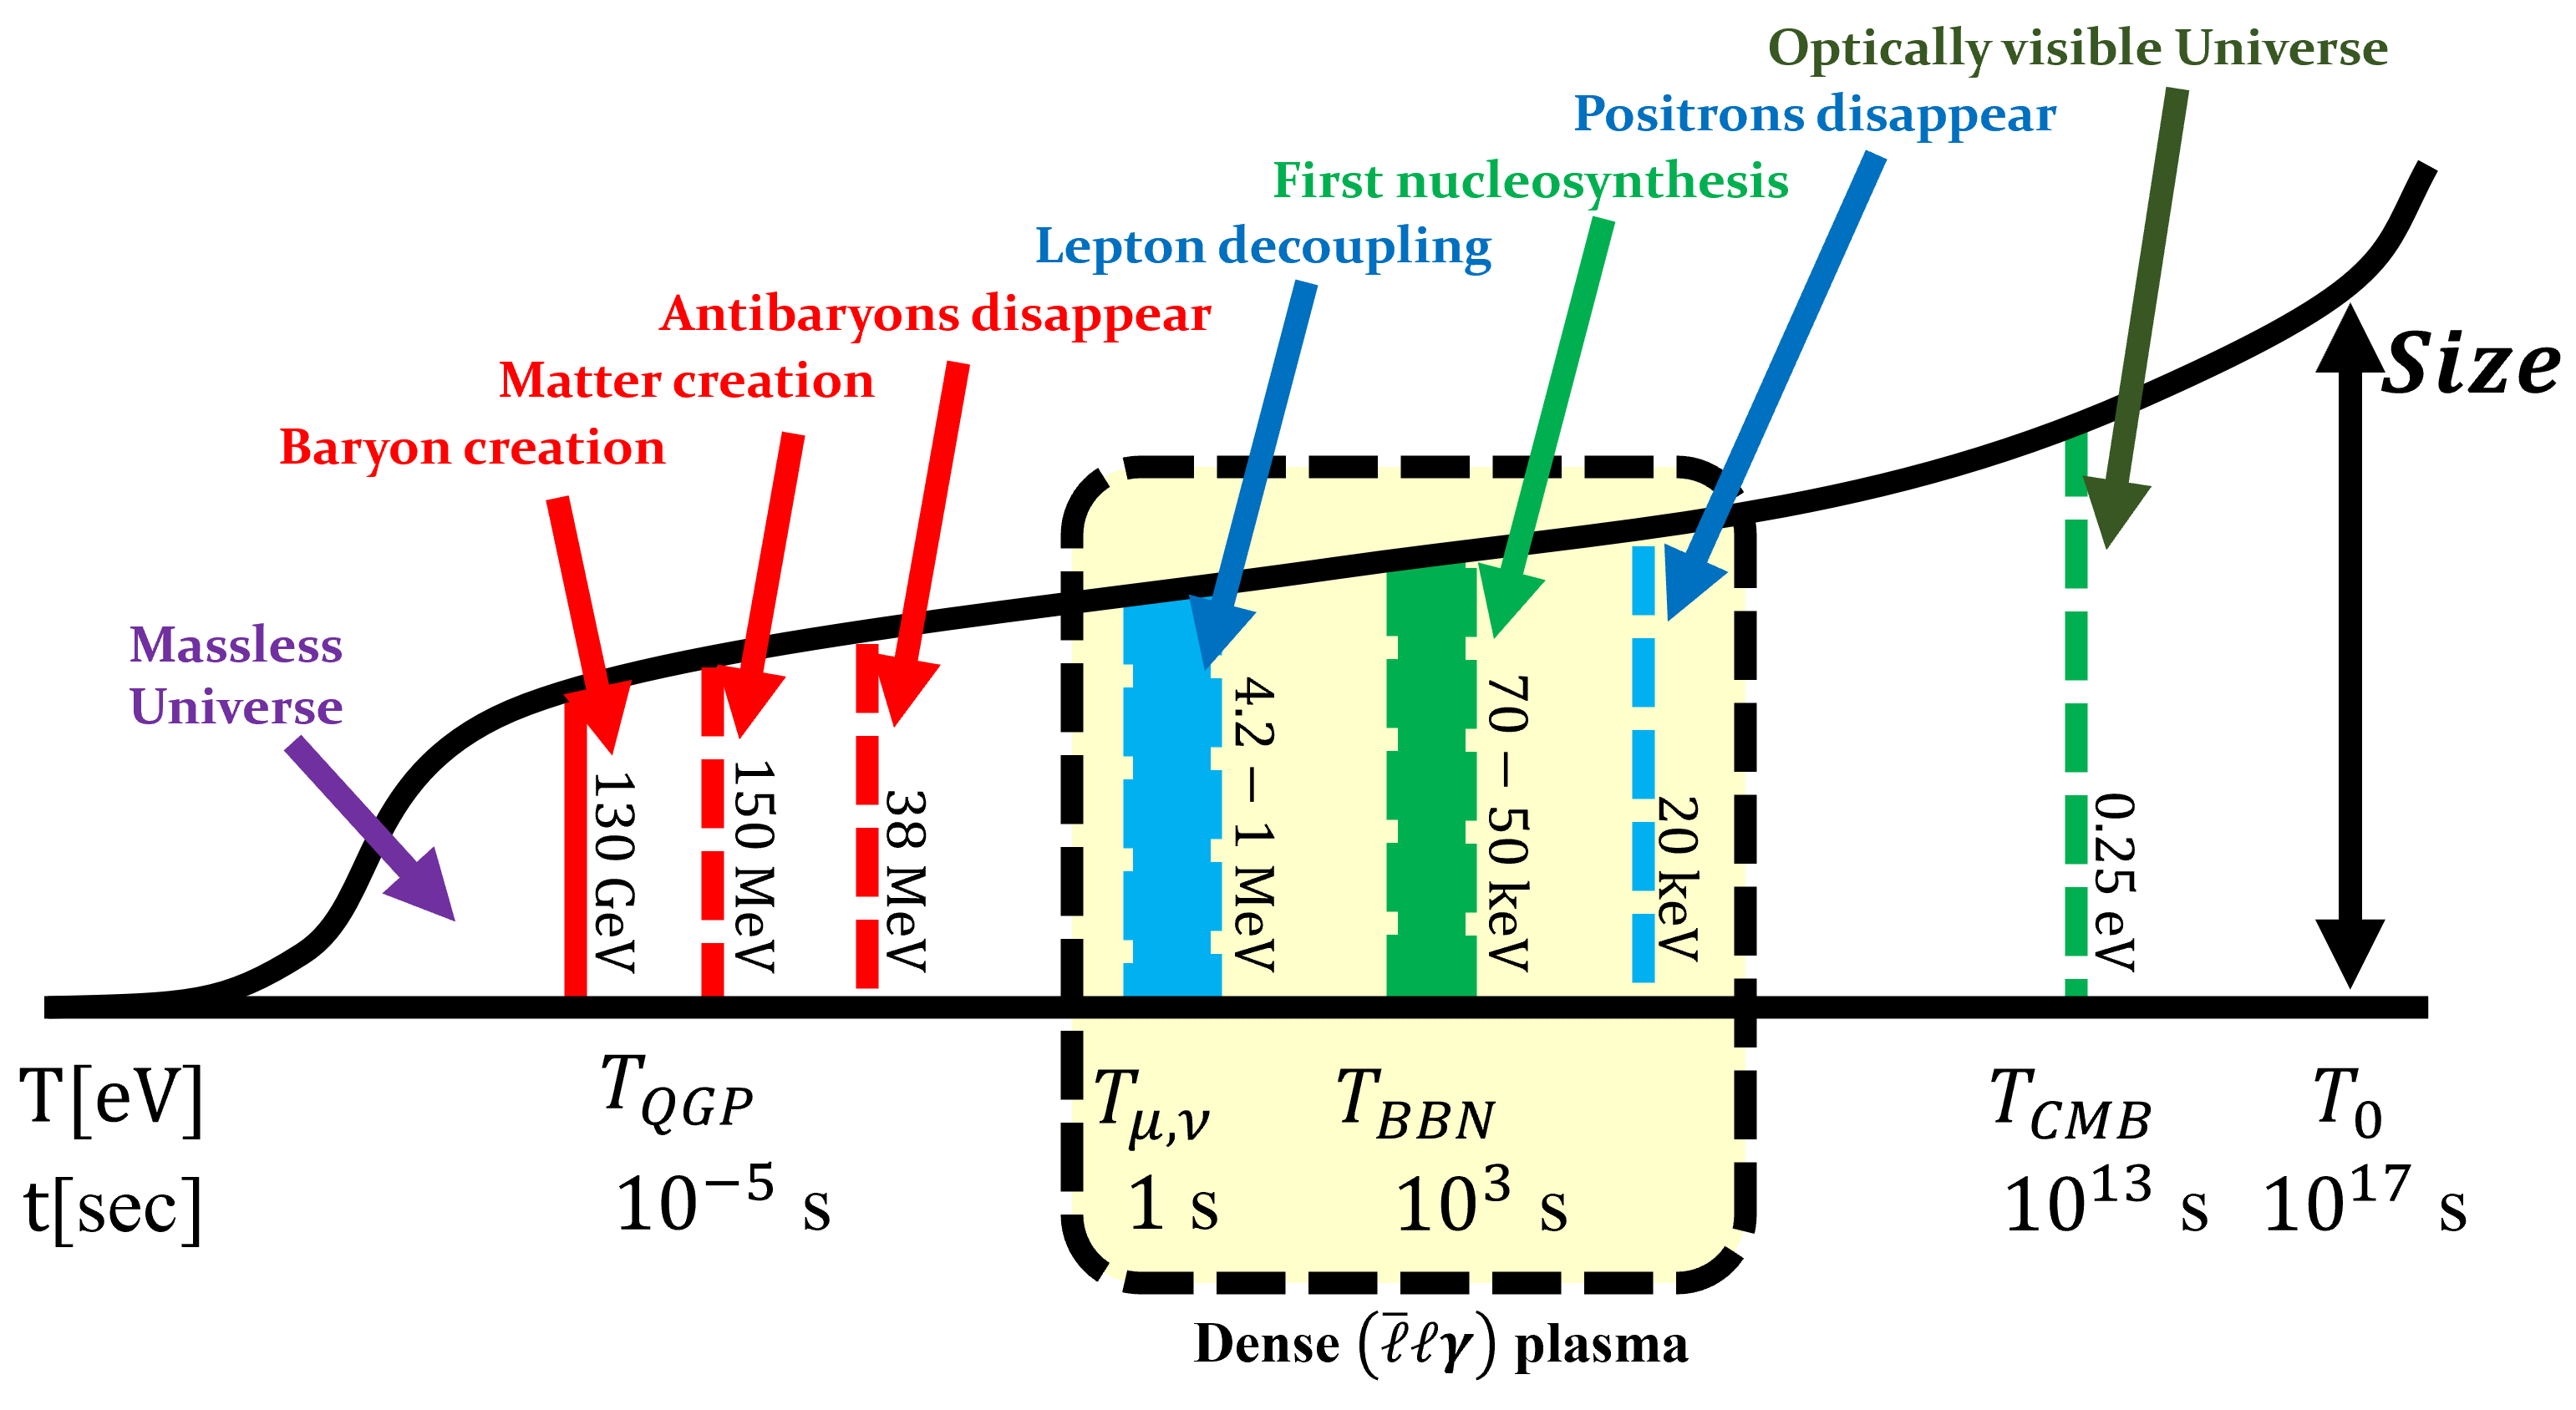
\includegraphics[width=0.95\linewidth]{plots/chap01intro/thesis_universe.png}
 \caption{A schematic of the universe's evolution since the Big Bang. The region of interest studied in this dissertation is emphasized (in the highlighted box) to contain a dense nearly charge neutral matter-antimatter plasma.}
 \label{fig:cosmo} 
\end{figure}
%%%%%%%%%%%%%%%%%%%%%%%%%%%%%%%%%%%%%%%

The scale factor $a(t)$ denotes the change of proper distances $L(t)$ over time as
\begin{gather}
    L(t)=L_{0}\frac{a_{0}}{a(t)}\rightarrow L(z)=L_{0}(1+z)\,,
\end{gather}
where $z$ is the redshift and $L_{0}$ the comoving length. In an expanding (or contracting) universe which is both homogeneous and isotropic, this implies volumes change with $V(t)=V_{0}/a^{3}(t)$ where $V_{0}=L_{0}^{3}$ is the comoving Cartesian volume. The evolutionary expansion of the universe is then traditionally defined in terms of the Hubble parameter $H(t)$ as follows
\begin{gather}
  \label{Friedmann:1} H(t)^{2}\equiv\left(\frac{\dot a}{a}\right)^2=\frac{8\pi G_{N}}{3}\rho_\mathrm{total},\qquad \rho_\mathrm{total}(t)=\rho_{\Lambda}+\rho_\mathrm{DM}(t)+\rho_\mathrm{Baryons}(t)+\ldots\\
  \label{Friedmann:2}
  \frac{\ddot a}{a}=-qH^2,\qquad 
q\equiv -\frac{a\ddot a}{\dot a^2},\qquad \dot H=-H^2(1+q).
\end{gather}
where $G_N$ is the Newtonian constant of gravitation. \req{Friedmann:1} and \req{Friedmann:2} are also known as the Friedmann equations. The total density $\rho_\mathrm{total}$ is the sum of all contributions from any form of matter, radiation or field. This includes but is not limited to: dark energy $(\Lambda)$, dark matter (DM), baryons (B), leptons $(\ell,\nu)$ and photons $(\gamma)$. Depending on the age of the universe, the relative importance of each group changes as each dilutes different under expansion with dark energy infamously remaining constant in density and accelerating the universe today.

The parameter $q$ is the cosmic deceleration parameter where for historical reasons expansion is slowing down for $q>0$. before the discovery of dark energy. The early universe was radiation dominated with $q = 1$, subsequently matter dominated with $q = 1/2$, and the contemporary universe is undergoing a transition from matter to dark energy dominated whereas the deceleration settles on the asymptotic value of $q = -1$; see~\cite{Rafelski:2013yka}.

We can consider the expansion to be an adiabatic process~\citep{Abdalla:2022yfr} which results in a smooth shifting of the relevant dynamical quantities. As the universe undergoes isotropic expansion, the temperature decreases as 
\begin{gather}
 \label{tscale}
 T(t)=T_{0}\frac{a_{0}}{a(t)}\rightarrow T(z)=T_{0}(1+z)\,,
\end{gather}
where $z$ is the redshift. The entropy within a comoving volume is kept constant until gravitational collapse effects become relevant. The comoving temperature $T_{0}$ is given by the the present CMB temperature $T_{0}=2.7{\rm\ K}\simeq2.3\times10^{-4}\eV$~\citep{Planck:2018vyg}, with contemporary scale factor $a_{0}=1$.

As the universe expands, redshift reduces the momenta of particles lowering their contribution to the energy content of the universe. This cosmological redshift is written as
\begin{alignat}{1}
  \label{Redshift} p_{i}(t) = p_{i,0}\frac{a_{0}}{a(t)}\,.
\end{alignat}
Momentum (and the energy of massless particles $E=pc$) scales with the same factor as temperature. The energy of massive free particles in the universe however scales differently based on their momentum (and thus temperature).

When hot and relativistic, particle energy scales inversely like radiation. As the particles transition to non-relativistic (NR) momenta, their energies scale with the inverse square of the scale factor
\begin{alignat}{1}
    \label{EScale} E(t) = E_{0}\frac{a_{0}}{a(t)}\xrightarrow{\mathrm{NR}}\  E_{0}\frac{a_{0}^{2}}{a(t)^{2}}\,.
\end{alignat}
This occurs because of the functional dependence of energy on momentum in the relativistic $E\sim p$ versus non-relativistic $E\sim p^{2}$ cases.